\documentclass{article}
\usepackage{amsmath}
\usepackage{enumerate}
\usepackage{listings}
\usepackage{moreverb}
\usepackage[margin=1in]{geometry}
\usepackage{graphicx}
\usepackage{dsfont}
\title{STA 360: Assignment 6}
\author{Michael Lin}

\begin{document}
\maketitle

\begin{enumerate}
\item
\begin{enumerate}
\item Given the p.d.f.
$$ p(x,y) \propto \mathds{1}(|x-y|<c)\mathds{1}(x,y\in (0,1)) $$
the Gibbs sampler for this distribution is:
$$ p(x|y) \propto \mathds{1}(|x-y|<c)\mathds{1}(x \in (0,1))$$
$$ p(y|x) \propto \mathds{1}(|x-y|<c)\mathds{1}(y \in (0,1))$$

\item See R code.

\item See below for graphs.

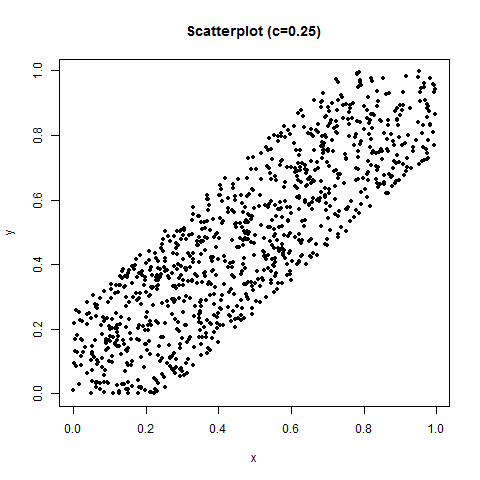
\includegraphics[scale=0.4]{scat_025.png}
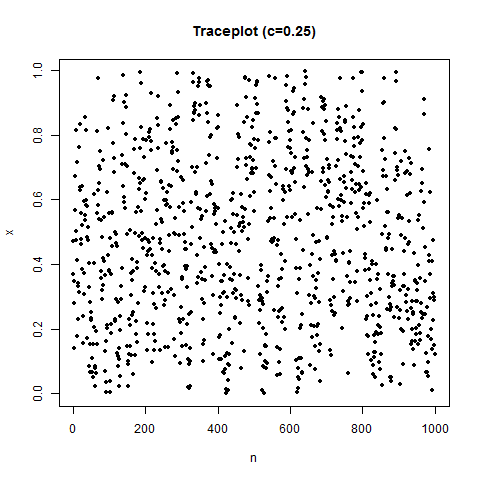
\includegraphics[scale=0.4]{trace_025.png} \\

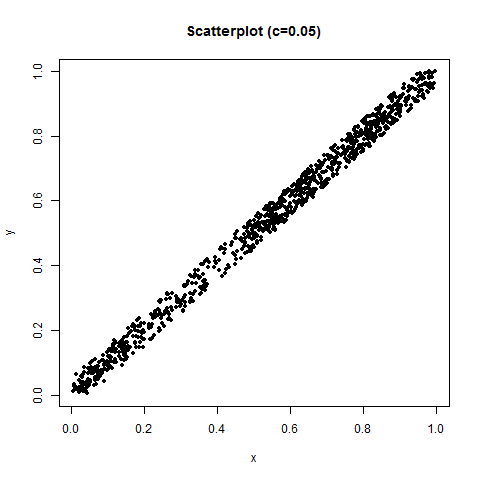
\includegraphics[scale=0.4]{scat_005.png}
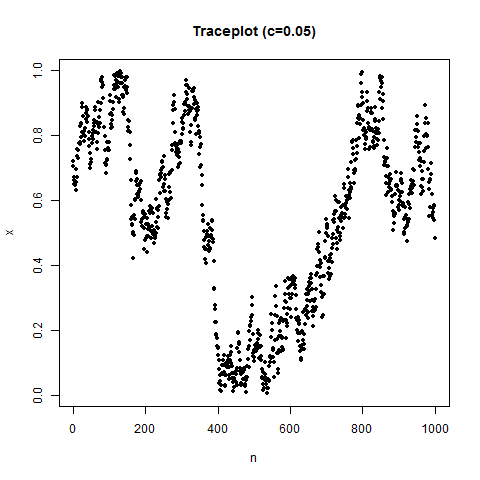
\includegraphics[scale=0.4]{trace_005.png} \\

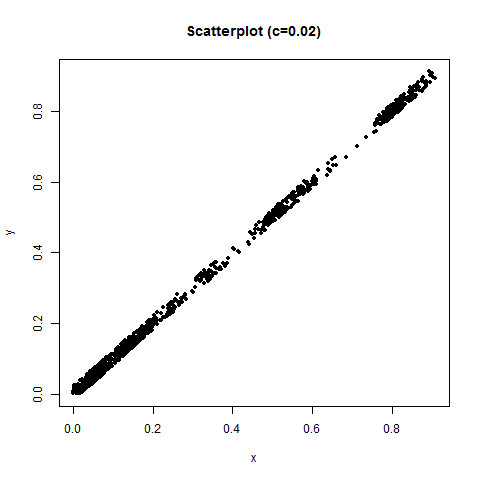
\includegraphics[scale=0.4]{scat_002.png}
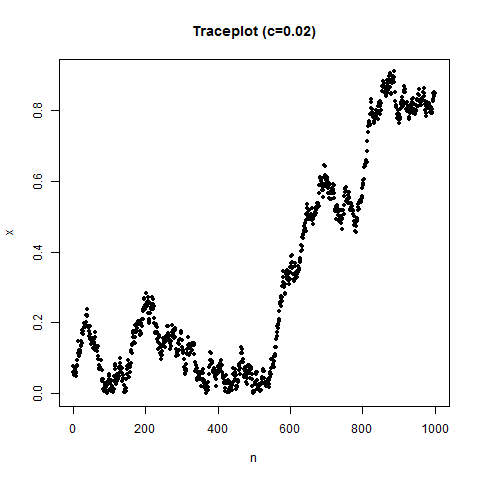
\includegraphics[scale=0.4]{trace_002.png}

\item The sampler will perform worse and worse as $c$ gets smaller because larger samples are needed to fully cover the probability space. Since $c$ is small, each sweep in the Gibbs sampling algorithm takes only a very small step (maximum of $c$). As a result, the distance covered by the sampler for $10^3$ steps is not sufficient to sample the entire probability space because $c$ is small. For instance, the sampler was only able to sample in a subset of the interval (0,1) for both $x$ and $y$. One easy way to ensure full coverage of probability space is taking larger number of samples, but this is not the most efficient method.
\end{enumerate}

\item

\begin{enumerate}
\item Given the p.d.f.
$$ p(u,v) = \mathds{1}(|v|<c/2)\mathds{1}(|v|<u<1-|v|) $$
the Gibbs sampler for this distribution is the following:
$$ p(u|v) = \mathds{1}(|v|<u<1-|v|) $$
$$ p(v) = \mathds{1}(|v|<c/2) $$

\item See R code.

\item See below for graphs.

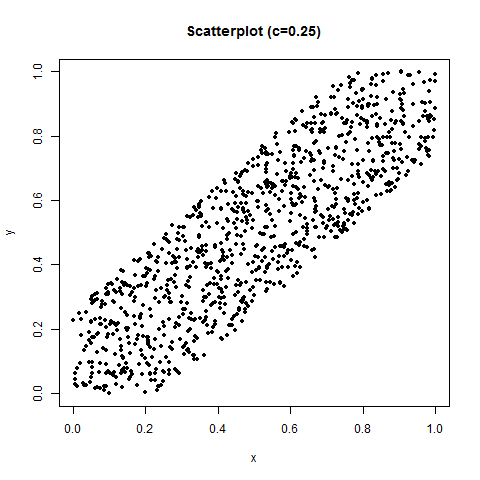
\includegraphics[scale=0.4]{scat_025x.png}
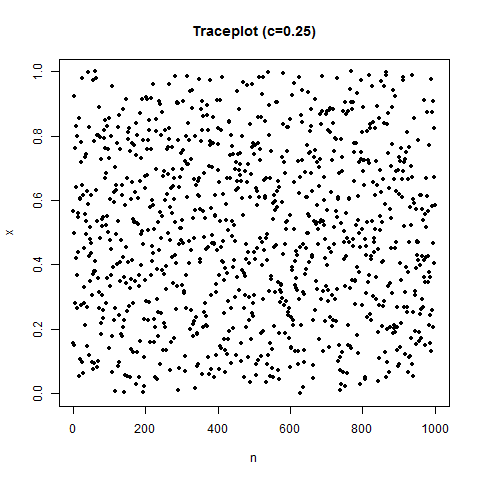
\includegraphics[scale=0.4]{trace_025x.png} \\

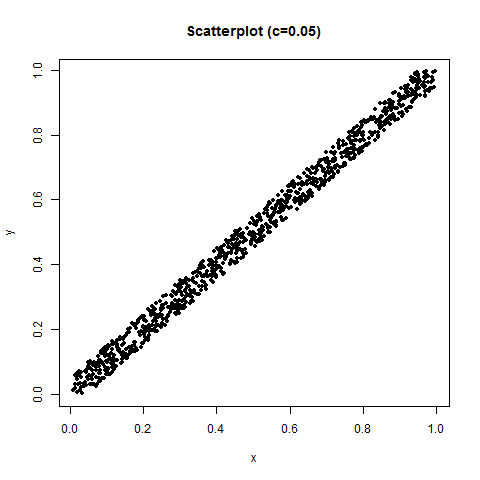
\includegraphics[scale=0.4]{scat_005x.png}
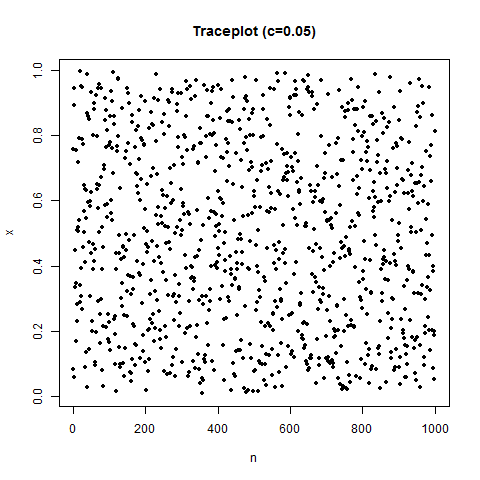
\includegraphics[scale=0.4]{trace_005x.png} \\

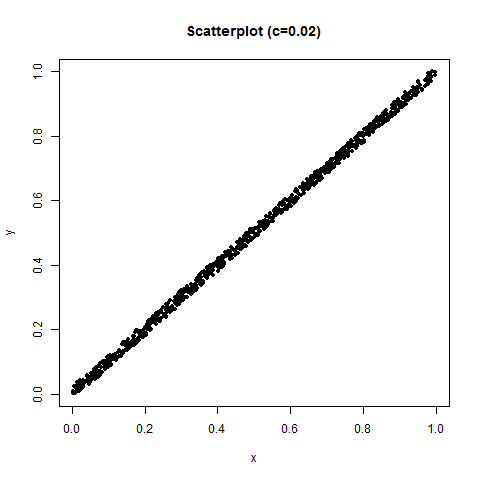
\includegraphics[scale=0.4]{scat_002x.png}
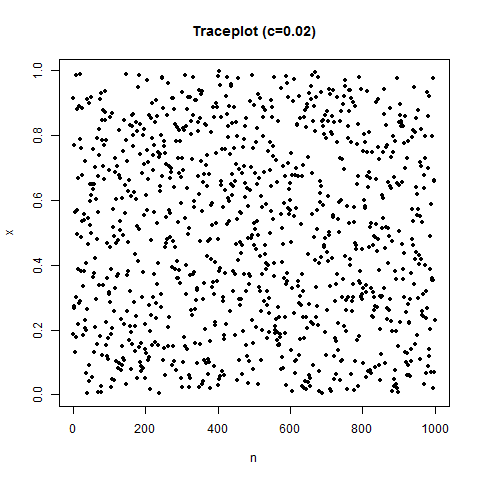
\includegraphics[scale=0.4]{trace_002x.png}

\item This sampler does not suffer from the issue as the previous one. Since the $v$'s don't have autocorrelation, each step is independent of $c$, which means the range of each step is not restrained by $c$. Therefore, the sampler is able to cover the entire probability space.

\end{enumerate}

\item

\begin{enumerate}
\item The full conditional $p(\beta | y,x,z,c)$:
\begin{align*}
p(\beta | y,x,z,c) &= p(\beta | x,z) \propto \Big[\prod\limits_{i=1}^{n} p(z_i | \beta,x_i)\Big]p(\beta|x_i) \\
&=\Big[\prod\limits_{i=1}^{n} \text{Normal}(z_i|\beta x_i,1) \Big]\text{Normal}(\beta|0,\tau_\beta^2) \\
&\propto \exp(-\frac{1}{2} \sum(z_i-\beta x_i)^2)\exp(-\frac{\beta^2}{2\tau_\beta^2}) \\
&= \exp(-\frac{1}{2} \sum(z_i^2-2\beta x_i z_i+\beta^2 x_i^2))\exp(-\frac{\beta^2}{2\tau_\beta^2}) \\
&\propto \exp(-\frac{1}{2}(\frac{\beta^2}{\tau_\beta^2}+\beta^2\sum x_i^2-2\beta\sum x_i z_i)) \\
&= \exp(-\frac{1}{2}(\beta^2(\frac{1}{\tau_\beta^2}+\sum x_i^2)-2\beta\sum x_i z_i)) \\
&\propto \exp(\frac{1}{2(\frac{1}{\tau_\beta^2}+\sum x_i^2)^{-1}}(\beta^2-2\beta \frac{\sum x_i z_i}{\frac{1}{\tau_\beta^2}+\sum x_i^2})) \\
&\propto \text{Normal}\Big(\frac{\sum x_i z_i}{\frac{1}{\tau_\beta^2}+\sum x_i^2}, (\frac{1}{\tau_\beta^2}+\sum x_i^2)^{-1}\Big)
\end{align*}

\item The full conditional $p(c|y,x,z,\beta)$:
\begin{align*}
p(c|y,x,z,\beta) &\propto \Big[\prod\limits_{i=1}^{n}p(y_i|c,z_i)\Big]p(c) \\
&= \Big[\prod\limits_{i=1}^{n}\mathds{1}(z_i>c)^{y_i}\mathds{1}(z_i<c)^{1-y_i}\Big]\text{Normal}(0,\tau_c^2) \\
&= \mathds{1}(\max(z_i:z_i<c)<c<\min(z_i:z_i>c))\text{Normal}(0,\tau_c^2)
\end{align*}
Note this is simply the normal distribution $\text{Normal}(0,\tau_c^2)$ bounded below by $\max(z_i:z_i<c)$ and bounded above by $\min(z_i:z_i>c)$.\\

The full conditional $p(z_i|y,x,z_{-i},\beta,c)$:
\begin{align*}
p(z_i|y,x,z_{-i},\beta,c) &\propto p(y|c,z_i)p(z_i|\beta,x_i) \\
&= \mathds{1}(z_i<c)^{1-y_i}\mathds{1}(z_i>c)^{y_i}\text{Normal}(\beta x_i,1)
\end{align*}
If $y_i=1$, this is simply the normal distribution $\text{Normal}(\beta x_i,1)$ bounded below by $c$. On the other hand, if $y_i=0$, then this is the same normal distribution bounded above by $c$.
\pagebreak
\item Below are the plots of the autocorrelation function for one run:

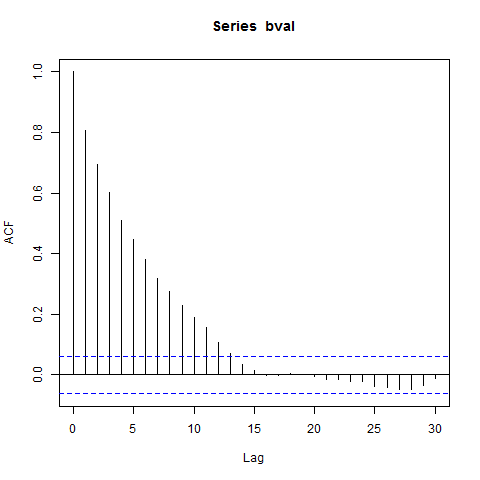
\includegraphics[scale=0.4]{bacf.png}
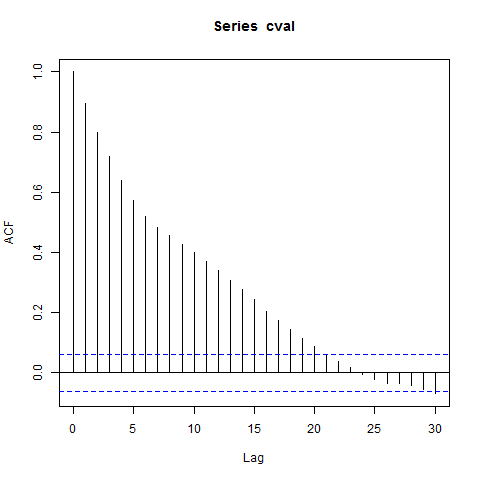
\includegraphics[scale=0.4]{acfc.png} \\

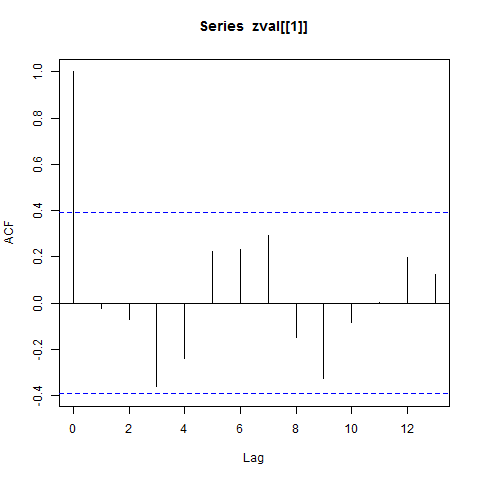
\includegraphics[scale=0.4]{acfz.png}\\

Also included here are the traceplots with running averages for $\beta$ and $c$ for 3 different initial values:

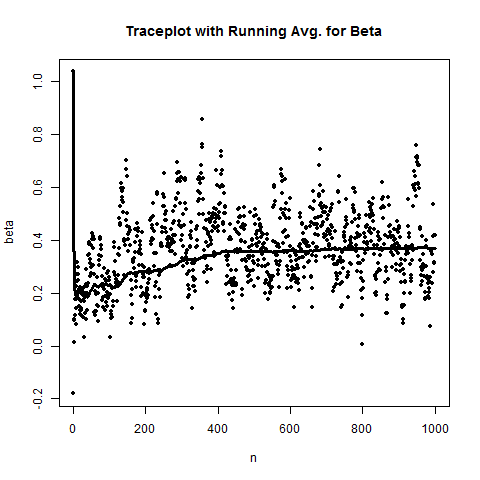
\includegraphics[scale=0.4]{mixb1.png}
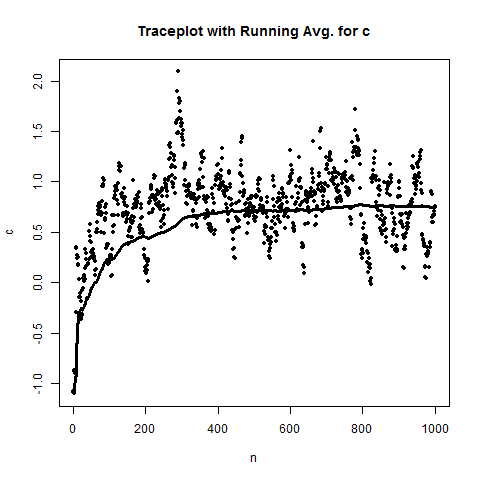
\includegraphics[scale=0.4]{mixc1.png} \\

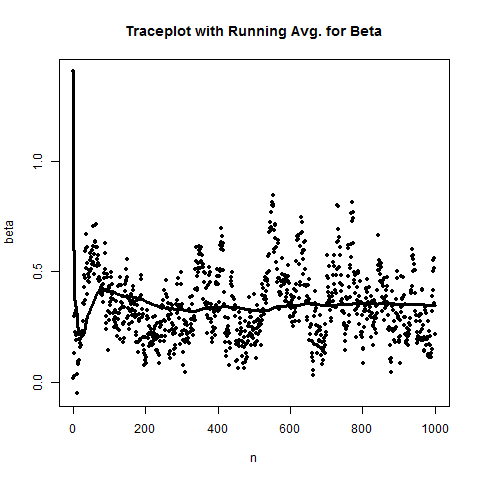
\includegraphics[scale=0.4]{mixb2.png}
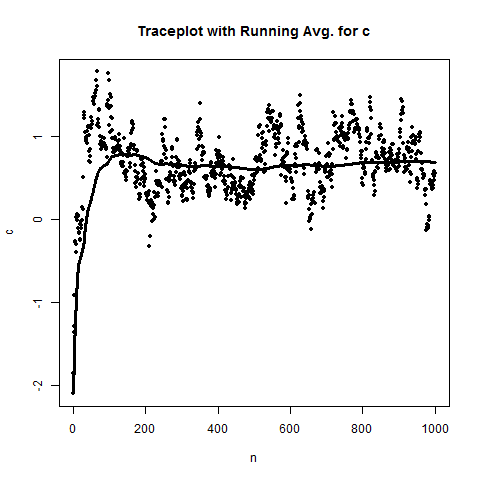
\includegraphics[scale=0.4]{mixc2.png} \\

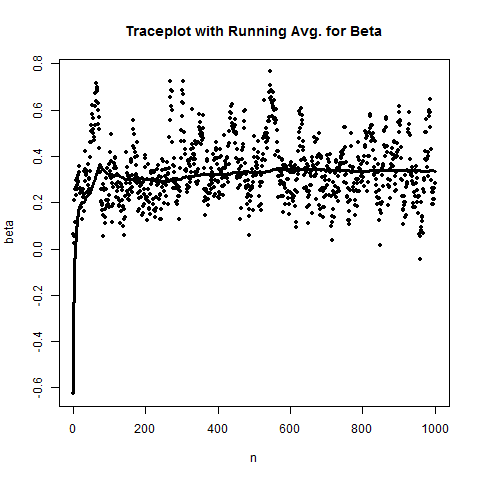
\includegraphics[scale=0.4]{mixb3.png}
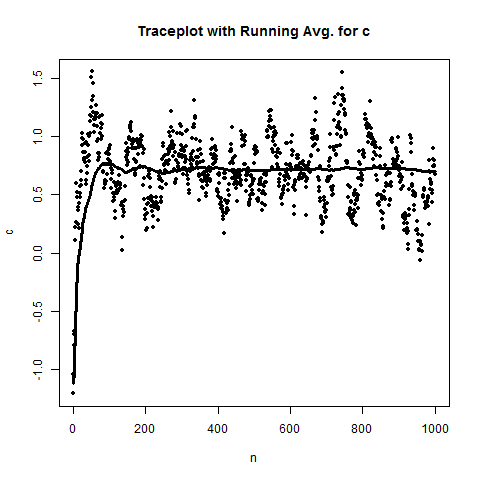
\includegraphics[scale=0.4]{mixc3.png} \\

Based on these trace plots, the Markov chain mixes relatively well because the sampler seems to traverse through regions of low probability and the running average converges. Therefore, the sampler seems to have reached the right distribution. In addition, autocorrelations for $\beta$ and $c$ decrease over successive sample, which also indicates that the sampler mixes well.

\item A 95\% posterior confidence interval for $\beta$ is:
$$[0.114, 0.630] $$
Furthermore, Pr$(\beta>0 | y,x) = 0.998$.
\end{enumerate}
\end{enumerate}

\pagebreak
R code for number 1:
\listinginput[1]{1}{assign6.r}

\pagebreak
R code for number 2:
\listinginput[1]{1}{assign6_2.r}

\pagebreak
R code for number 3:
\listinginput[1]{1}{divorce.r}

\end{document}